%%%%%%%%%%%%%%%%%%%%%%%%%%%%%%%%%%%%%%%%%%%%%%%%%%%%%%%%%%%%%%%%%%%%%%%%%%%%%%%
% Chapter 'Adsorption - 1-Butene - zeolite pellet 13X'
%%%%%%%%%%%%%%%%%%%%%%%%%%%%%%%%%%%%%%%%%%%%%%%%%%%%%%%%%%%%%%%%%%%%%%%%%%%%%%%
\subsection{Zeolite pellet 13X}
%
%%%%%%%%%%%%%%%%%%%%%%%%%%%%%%%%%%%%%%%%%%%%%%%%%%%%%%%%%%%%%%%%%%%%%%%%%%%%%%%
%%%%%%%%%%%%%%%%%%%%%%%%%%%%%%%%%%%%%%%%%%%%%%%%%%%%%%%%%%%%%%%%%%%%%%%%%%%%%%%
\subsubsection{Toth - ID 1}
%
\begin{tabular}[l]{|lp{11.5cm}|}
\hline
\addlinespace

\textbf{Sorbent:} & zeolite pellet \\
\textbf{Subtype:} & 13X \\
\textbf{Refrigerant:} & 1-Butene \\
\textbf{Equation:} & Toth \\
\textbf{ID:} & 1 \\
\textbf{Reference:} & Lamia, Nabil; Wolff, Luc; Leflaive, Philibert; Leinekugel‐Le‐Cocq, Damien; Sá Gomes, Pedro; Grande, Carlos A.; Rodrigues, Alírio E. (2008): Equilibrium and Fixed Bed Adsorption of 1‐Butene, Propylene and Propane Over 13X Zeolite Pellets. In: Separation Science and Technology 43 (5), S. 1124–1156. DOI: 10.1080/01496390801888136. \\
\textbf{Comment:} & None \\

\addlinespace
\hline
\end{tabular}
\newline

\textbf{Properties of sorbent:}
\newline
%
\begin{longtable}[l]{lll}
\toprule
\addlinespace
\textbf{Property} & \textbf{Unit} & \textbf{Value} \\
\addlinespace
\midrule
\endhead
\bottomrule
\endfoot
\bottomrule
\endlastfoot
\addlinespace

Diameter of crystal & \si{\milli\meter} & 0.001\\
Diameter of pore & \si{\milli\meter} & 0.0000005\\
Diameter of extrudate & \si{\milli\meter} & 0.8\\
Porosity of pellet & - & 0.395\\
Pellet density & \si{\kilogram\per\cubic\meter} & 1357\\

\addlinespace\end{longtable}

\textbf{Equation and parameters:}
\newline
%
Loading $w$ in $\si{\kilogram\per\kilogram}$ is calculated depending on pressure $p$ in $\si{\pascal}$ and temperature $T$ in $\si{\kelvin}$ by:
%
\begin{equation*}
\begin{split}
w &=& \frac{w_\mathrm{sat} b^{m} p}{\left( 1 + b^{r} p^{n} \right)^{\nicefrac{1}{n}}} & \quad\text{, and} \\
b &=& b_0 \exp\left( \frac{Q^{*}}{T} \right) & \quad\text{, and} \\
n &=& n_0 + \nicefrac{c}{T} & \quad\text{, and} \\
r &=& \begin{cases} n & \quad \text{if } r^{*} < 0 \\ r^{*}  & \quad \text{else} \end{cases} & \quad\text{.}
\end{split}
\end{equation*}
%
The parameters of the equation are:
%
\begin{longtable}[l]{lll|lll}
\toprule
\addlinespace
\textbf{Par.} & \textbf{Unit} & \textbf{Value} &	\textbf{Par.} & \textbf{Unit} & \textbf{Value} \\
\addlinespace
\midrule
\endhead

\bottomrule
\endfoot
\bottomrule
\endlastfoot
\addlinespace

$b_0$ & $\si{\per\pascal}$ & 2.500000000e-10 & $Q^{*}$ & $\si{\kelvin}$ & 6.542816114e+03 \\
$c$ & $\si{\kelvin}$ & 0.000000000e+00 & $r^{*}$ & - & -1.000000000e+00 \\
$m$ & - & 1.000000000e+00 & $w_\mathrm{sat}$ & $\si{\kilogram\per\kilogram}$ & 1.178310000e-01 \\
$n_0$ & - & 4.520000000e-01 & & & \\

\addlinespace\end{longtable}

\textbf{Validity:}
\newline
Equation is approximately valid for $0.0 \si{\pascal} \leq p \leq 110050.0 \si{\pascal}$,  $333.0 \si{\kelvin} \leq T \leq 393.0 \si{\kelvin}$, and $0.0 \si{\kilogram\per\kilogram} \leq w \leq 0.1155866 \si{\kilogram\per\kilogram}$.
\newline

\textbf{Visualization:}
%
\begin{figure}[!htp]
{\noindent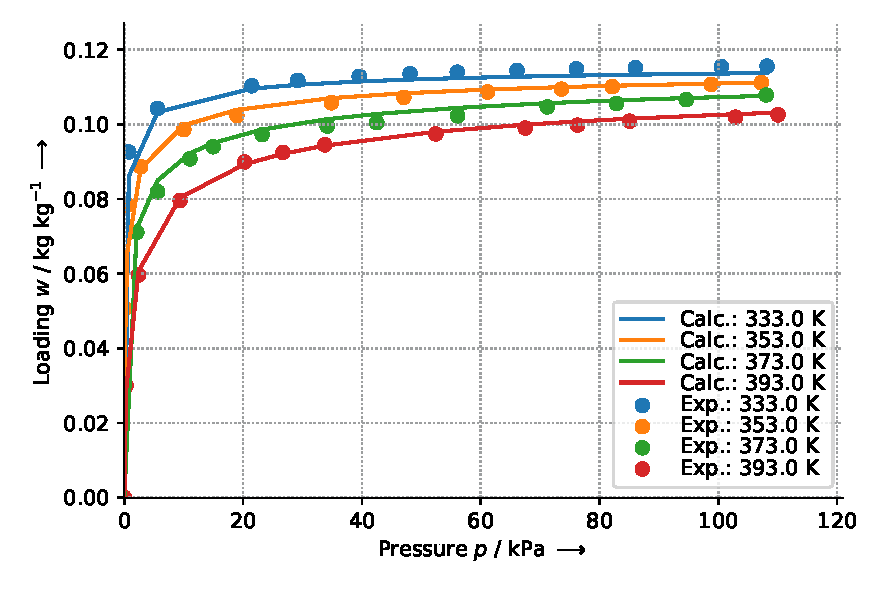
\includegraphics[height=10cm, keepaspectratio]{figs/ads/ads_1-Butene_zeolite_pellet_13X_Toth_1.pdf}}
\end{figure}
%

To generate the figure, the following refrigerant functions were selected:
\begin{itemize}
\item Vapor pressure: VaporPressure\_EoS1 - ID 1
\item Saturated liquid density: NoSaturatedLiquidDensity - ID 1
\end{itemize}

The uncertainity of the experimental data is:
\begin{itemize}
\item Data source $\,\to\,$ Data was taken from figure
\item Pressure, absolute, in $\si{\pascal}$ $\,\to\,$ 50
\item Temperature, absolute, in $\si{\kelvin}$ $\,\to\,$ 0.1
\end{itemize}

The mean absolute percentage error (MAPE) between the experimental and calculated data results in 1.85\%.
\FloatBarrier
\newpage
%%%%%%%%%%%%%%%%%%%%%%%%%%%%%%%%%%%%%%%%%%%%%%%%%%%%%%%%%%%%%%%%%%%%%%%%%%%%%%%
